\documentclass[12pt, a4paper]{report}
\usepackage[utf8]{inputenc}
\usepackage{graphicx}
\usepackage{hyperref}
\usepackage{listings}
\usepackage{xcolor}
\usepackage{geometry}
\usepackage{fancyhdr}
\usepackage{tikz}
\usetikzlibrary{shapes.geometric, arrows, positioning}

\geometry{margin=1in}
\hypersetup{colorlinks=true, linkcolor=blue, urlcolor=blue}

\title{Model Context Protocol (MCP) Capstone Project}
\author{University Assistant Demonstration System}
\date{March 2026}

\begin{document}

\maketitle
\tableofcontents
\newpage

\chapter{Introduction}

\section{Project Overview}
This capstone project demonstrates the implementation of a Model Context Protocol (MCP) system that integrates a React frontend with an MCP server architecture. The system showcases academic assistant capabilities through structured tool execution and protocol compliance.

\section{Objectives}
\begin{itemize}
    \item Implement MCP protocol compliance for tool discovery and execution
    \item Demonstrate layered architecture with clear separation of concerns
    \item Provide academic assistant functionality (GPA calculation, exam scheduling)
    \item Create responsive React frontend with modern UI components
    \item Establish robust error handling and logging pipeline
\end{itemize}

\chapter{System Architecture}

\section{Architecture Overview}
The system follows a four-layer architecture:
\begin{itemize}
    \item \textbf{Model Layer}: Tool selection logic based on user queries
    \item \textbf{Context Layer}: System context management (session, environment, timestamps)
    \item \textbf{Tool Layer}: MCP protocol-based tool discovery and execution
    \item \textbf{Execution Layer}: Actual tool implementation
\end{itemize}

\section{Data Flow}
\begin{center}
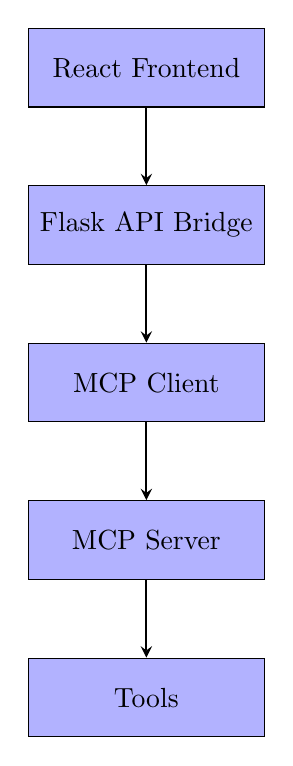
\begin{tikzpicture}[node distance=2cm]
\tikzstyle{process} = [rectangle, minimum width=3cm, minimum height=1cm, text centered, draw=black, fill=blue!30]
\tikzstyle{arrow} = [thick,->,>=stealth]

\node (frontend) [process] {React Frontend};
\node (flask) [process, below of=frontend] {Flask API Bridge};
\node (mcp) [process, below of=flask] {MCP Client};
\node (server) [process, below of=mcp] {MCP Server};
\node (tools) [process, below of=server] {Tools};

\draw [arrow] (frontend) -- (flask);
\draw [arrow] (flask) -- (mcp);
\draw [arrow] (mcp) -- (server);
\draw [arrow] (server) -- (tools);
\end{tikzpicture}
\end{center}

\chapter{Implementation Details}

\section{Frontend Implementation}
\subsection{Technology Stack}
\begin{itemize}
    \item React 18 with TypeScript
    \item TailwindCSS for styling
    \item Framer Motion for animations
    \item Radix UI components
    \item Lucide Icons
    \item Vite build tool
\end{itemize}

\subsection{Key Components}
\begin{itemize}
    \item \textbf{Dashboard.tsx}: Main user interface
    \item \textbf{API Service Layer}: Handles communication with Flask backend
    \item \textbf{UI Components}: Reusable components for consistent design
\end{itemize}

\section{Backend Implementation}
\subsection{Flask API Bridge}
The Flask API serves as the bridge between the React frontend and MCP pipeline:
\begin{itemize}
    \item Handles HTTP requests from frontend
    \item Manages user sessions and context
    \item Implements retry mechanism for robustness
    \item Provides CORS support for cross-origin requests
\end{itemize}

\subsection{MCP Server}
The MCP server implements the Model Context Protocol:
\begin{itemize}
    \item Tool discovery and registration
    \item Structured input/output schemas
    \item Protocol compliance for tool execution
    \item Academic tool implementations
\end{itemize}

\chapter{Available Tools}

\section{GPA Calculator}
\begin{itemize}
    \item \textbf{Tool Name}: \texttt{calculate\_gpa}
    \item \textbf{Description}: Calculate GPA from letter grades
    \item \textbf{Input}: Array of letter grades (A, B, C, D, F)
    \item \textbf{Output}: Calculated GPA value
    \item \textbf{Sample Query}: "calculate my gpa"
\end{itemize}

\section{Exam Schedule Checker}
\begin{itemize}
    \item \textbf{Tool Name}: \texttt{check\_exam\_schedule}
    \item \textbf{Description}: Get exam schedule for a course
    \item \textbf{Input}: Course code string
    \item \textbf{Output}: Exam date and time information
    \item \textbf{Sample Query}: "when is my exam"
\end{itemize}

\section{Course Registration}
\begin{itemize}
    \item \textbf{Tool Name}: \texttt{register\_course}
    \item \textbf{Description}: Register for a new course
    \item \textbf{Input}: Course code, name, credits, semester
    \item \textbf{Output}: Registration confirmation
\end{itemize}

\chapter{API Response Format}

\section{MCP Response Structure}
The system returns structured responses in the MCPResponse format:

\begin{verbatim}
{
  "context": {
    "timestamp": "2026-03-09T05:08:47.644482",
    "user_session": "demo-user-123",
    "environment": "academic-demonstration",
    "platform": "windows",
    "system_status": "ready"
  },
  "tools": ["calculate_gpa", "check_exam_schedule"],
  "selected_tool": "calculate_gpa",
  "parameters": {
    "grades": ["A", "B", "A"]
  },
  "result": {
    "text": "Calculated GPA: 3.67"
  }
}
\end{verbatim}

\section{Pipeline Flow}
\begin{enumerate}
    \item \textbf{User Query}: React frontend sends query to Flask API
    \item \textbf{Context Loading}: System loads session context
    \item \textbf{Tool Discovery}: MCP client discovers available tools
    \item \textbf{Model Selection}: Model layer selects appropriate tool
    \item \textbf{MCP Execution}: Tool executed via MCP protocol
    \item \textbf{Response Return}: Structured response returned to frontend
\end{enumerate}

\chapter{Deployment and Installation}

\section{Prerequisites}
\begin{itemize}
    \item Python 3.11+
    \item Node.js 18+
    \item npm package manager
\end{itemize}

\section{Installation Steps}
\subsection{Python Dependencies}
\begin{verbatim}
pip install mcp fastapi flask flask-cors uvicorn
\end{verbatim}

\subsection{Frontend Dependencies}
\begin{verbatim}
cd frontend
npm install
cd ..
\end{verbatim}

\section{Running the System}
\subsection{Step 1: Start MCP Server}
\begin{verbatim}
cd mcp_project
python server.py
\end{verbatim}

\subsection{Step 2: Start Flask Backend}
\begin{verbatim}
cd ..
python api_flask.py
\end{verbatim}

\subsection{Step 3: Start React Frontend}
\begin{verbatim}
cd frontend
npm run dev
\end{verbatim}

\section{Access Points}
\begin{itemize}
    \item \textbf{Frontend}: http://localhost:5173
    \item \textbf{Backend API}: http://localhost:8000
    \item \textbf{API Endpoint}: POST http://localhost:8000/ask
\end{itemize}

\chapter{Testing and Validation}

\section{Sample Queries}
\begin{itemize}
    \item "calculate my gpa"
    \item "what's my gpa"
    \item "check my grades"
    \item "when is my exam"
    \item "exam schedule"
    \item "check exam for AI407"
\end{itemize}

\section{Logging Pipeline}
The system provides comprehensive logging at each pipeline step:
\begin{verbatim}
Context loaded
Tools discovered: ['calculate_gpa', 'check_exam_schedule']
Model selected tool: calculate_gpa
Executing tool via MCP
Returning response to frontend
\end{verbatim}

\chapter{Technical Achievements}

\section{MCP Compliance}
\begin{itemize}
    \item Complete MCP protocol implementation
    \item Dynamic tool discovery
    \item Structured input/output schemas
    \item Protocol-compliant error handling
\end{itemize}

\section{Architecture Benefits}
\begin{itemize}
    \item Clear layer separation
    \item Modular design for extensibility
    \item Session management and context preservation
    \item Retry mechanism for reliability
\end{itemize}

\section{User Experience}
\begin{itemize}
    \item Responsive React interface
    \item Real-time feedback
    \item Modern UI components
    \item Cross-browser compatibility
\end{itemize}

\chapter{Conclusion}

\section{Project Summary}
This capstone project successfully demonstrates a complete Model Context Protocol implementation with academic assistant capabilities. The system showcases modern web development practices, protocol compliance, and robust architecture design.

\section{Key Achievements}
\begin{itemize}
    \item Full MCP protocol implementation
    \item Four-layer architecture with clear separation
    \item Responsive React frontend with TypeScript
    \item Robust Flask API bridge with session management
    \item Academic tools with structured schemas
    \item Comprehensive error handling and logging
\end{itemize}

\section{Future Enhancements}
\begin{itemize}
    \item Additional academic tools (gradebook, attendance)
    \item Database integration for persistent storage
    \item Authentication and authorization
    \item Mobile application development
    \item Performance optimization and caching
\end{itemize}

\chapter{References}

\begin{thebibliography}{9}
\bibitem{mcp} Model Context Protocol Specification, \url{https://modelcontextprotocol.io/}
\bibitem{mcp-python} MCP Python Library, \url{https://github.com/modelcontextprotocol/python-sdk}
\bibitem{react} React Documentation, \url{https://react.dev/}
\bibitem{flask} Flask Documentation, \url{https://flask.palletsprojects.com/}
\bibitem{tailwind} TailwindCSS Documentation, \url{https://tailwindcss.com/}
\end{thebibliography}

\appendix
\chapter{Project Structure}

\begin{verbatim}
capstone-lab mid/
├── frontend/                    # React + Tailwind UI
│   ├── src/
│   │   ├── components/          # UI components
│   │   ├── pages/              # Dashboard page
│   │   └── services/          # API service layer
│   └── package.json
├── mcp_project/                # MCP Implementation
│   ├── mcp_server/            # MCP server components
│   ├── client/                 # MCP client layer
│   ├── model/                  # Model layer (tool selection)
│   ├── execution/              # Tool execution layer
│   ├── server.py              # MCP server
│   ├── client_bridge.py       # MCP client bridge
│   └── _mcp_worker.py        # MCP pipeline worker
├── api_flask.py               # Flask API bridge
└── README.md
\end{verbatim}

\end{document}
